\chapter{Related Work}
In this section, we first review a set of work that aims to enable touch interaction on everyday surfaces and objects. Then we dive deeper into prior work in the field of capacitive sensing closely related to \textit{FlexTouch} to better position our work in the related literature.

\section{Touch Interaction on Everyday Surfaces and Objects}
Researchers have explored various methods and techniques to enable interactive interfaces on everyday surfaces and objects. One popular method to enable touch interactions, as shown in Fig ~\ref{fig:cv-large-scale-interaction} is by projecting 2D user interfaces onto a surface and then recognize user interaction via computer vision technique ~\cite{pinhanez2001everywhere, Fails-2002-Light-Widgets, Wilson-2010-Light-Space, Xiao-WorldKit}. These solutions can support large-scale interactions which are suitable for fixed infrastructure. However, its power consumption and form factor are still challenging for everyday mobile scenarios.  Furthermore, the cost of the toolkit as well as the difficulty of setup also makes it far way from being popularized to ordinary people. 

% \begin{figure}[ht]
%     \centering
% 	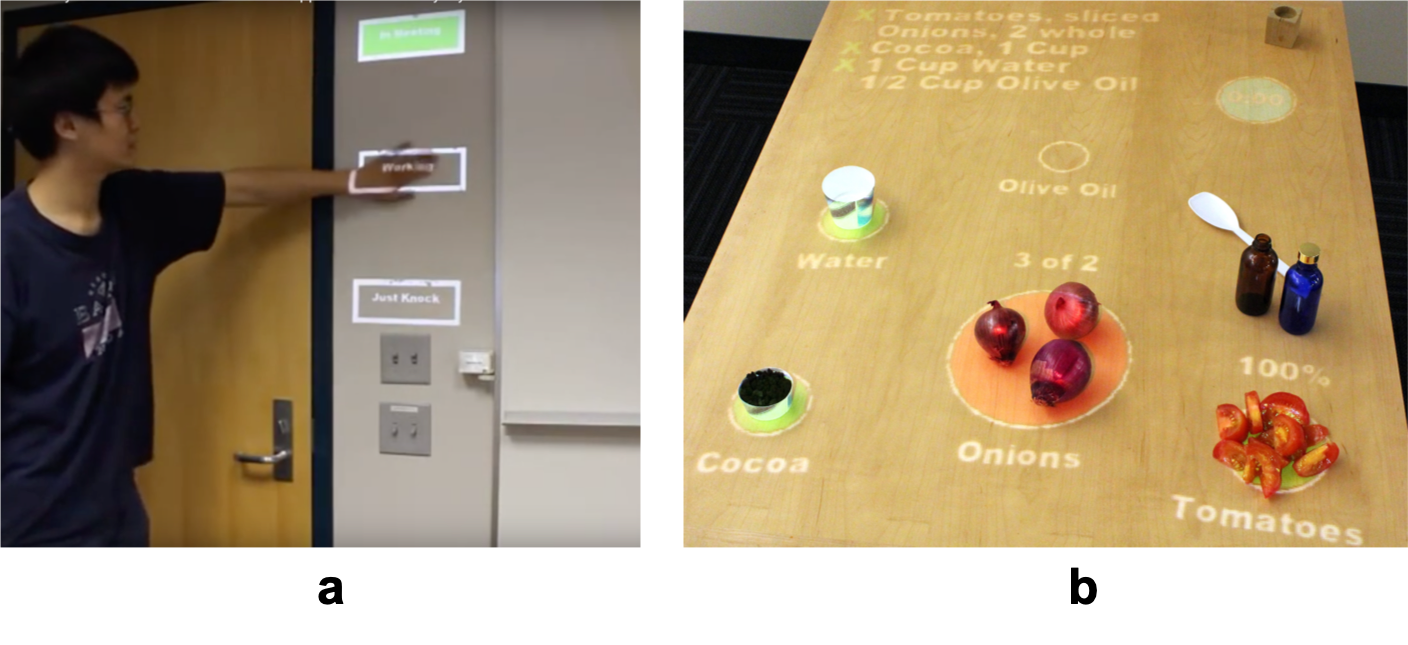
\includegraphics[width=0.70\columnwidth]{figures/cv-large-scale-sensing.png}
% 	\setlength{\belowcaptionskip}{-6pt}
%     \caption{Example applications of vision-based large-scale interaction: a) notification message application. b) Kitchen application.}
%     \label{fig:cv-large-scale-interaction}
% \end{figure}

Touch interaction can also be supported by acoustic sensing Ono's work is based on the difference of resonate properties of different objects ~\cite{Ono-Touch-and-Activate}. By training a model for recognizing different acoustic wave patterns, it is able to distinguish various touch events. Researchers have explored recognizing a discrete set of touch events on everyday objects such as windows ~\cite{Paradiso-2002-Window}, desktops, and other surfaces ~\cite{Harrison-2008-Scratch-iput}. However, these approaches only apply towards a small set of touch inputs like tapping or scratching on various materials. However, these approaches cannot live without dedicated sensing platforms to collect and transmiting acoustic data from objects. 

% \begin{figure}[ht]
%     \centering
% 	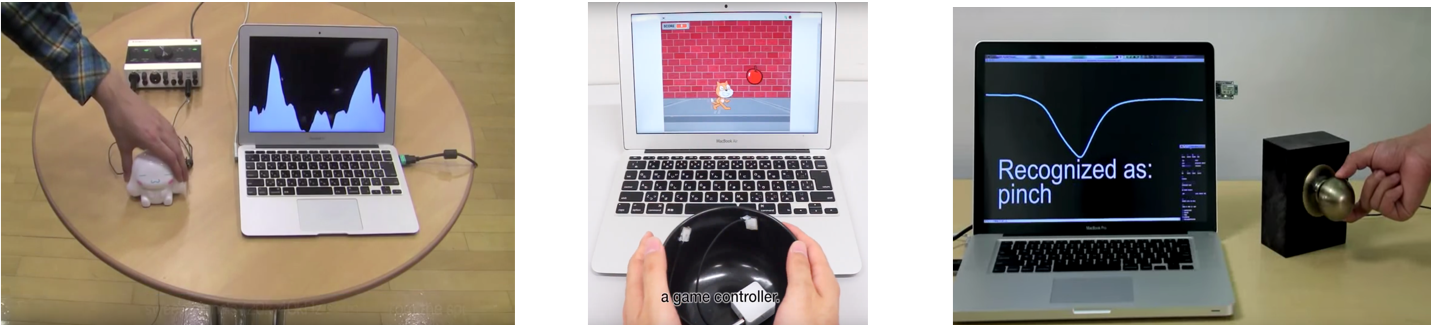
\includegraphics[width=0.70\columnwidth]{figures/acoustic-sensing.png}
% 	\setlength{\belowcaptionskip}{-6pt}
%     \caption{Touch & Activate: Adding interactivity of existing objects using active acoustic sensing}
%     \label{fig:acoustic-sensing}
% \end{figure}

Another popular method is electromagnetic sensing. \textit{SmartSkin} enabled multi-touch interaction on surfaces using a mesh-shaped capacitive sensor grid ~\cite{Rekimoto-SmartSkin}. \textit{Electrick} ~\cite{Zhang-Electrick} and \textit{Pulp Nonfiction} ~\cite{Zhang-pulp} enabled touch input on everyday surfaces and objects using Electric Field Tomography (EIT) with coated conductive materials on everyday surfaces and objects. \textit{Touche} ~\cite{Sato-Touche} enhances touch interface on the human body or everyday objects by measuring the electrical profiles with a frequency-sweep signal. \textit{Midas} ~\cite{Savage-2012-Midas} fabricated customized capacitive touch sensors to prototyping interactive object with a circuit board milling machine. \textit{Wall++} ~\cite{Zhang-wall} enabled large-scale touch interaction on the wall for activity recognition. Other prior work also explored printing custom-shaped capacitive sensors ~\cite{gong2014printsense,olberding2015foldio,olberding2014printscreen,vadgama2017flexy}. These prior works demonstrated very promising results, however, they rely heavily on dedicated sensing platforms and customized embedded systems to provide power supply, external sensors, signal processing, and communication modules. These requirements create barriers for end-users to easily fabricate customized touch interfaces.

\section{Capacitive Touch Interaction Sensing beyond Touchscreens}
Capacitive sensing was introduced into the field of HCI over two decades ago. Recently, Grosse-Puppendahl and his colleagues reviewed and summarized past researches related to capacitive sensing theories and techniques ~\cite{Grosse-Puppendahl-capacitive}. Among all the capacitive sensing methods, shunt mode sensing is the most widely spread approach in implementing modern capacitive touchscreens. The touch panel consists of multiple layers above the display screen with all the sensing nodes oriented in a row-column matrix. Each node is a high-resolution continuous capacitance measurement sensor. Obtaining the low-level capacitive data from the touchscreen provides us with more capability beyond binary finger touch sensing. Similar to our approach, \textit{BodyPrint} ~\cite{Holz-bodyprint} and \textit{CapAuth} ~\cite{Guo2015} combined capacitive touchscreens with machine learning classifiers to provide authentication and even identification of users. \textit{PalmTouch} enabled the palm as an additional input modality to enhance mobile interaction ~\cite{Le-palmtouch}. Researchers also explored the potential of using the raw capacitive data of touchscreens to support sensing of tangible 3D-printed gadgets on top of the screen ~\cite{Chan-CapStones, Schmitz2017, Schmitz2018}. While these prior works share the same raw capacitance signal as our approach, we focus on fabricating conductive interfaces to support large-scale, flexible touch interfaces on the ambient surfaces connected to touchscreens.

Modern mobile devices are embedded with rich sensors and actuators. Researchers have explored approaches and techniques enhancing the interaction around mobile devices with customized sensors via active and passive techniques. Researchers have explored attaching capacitive sensors to mobile devices to enable interactive user applications. iGrasp ~\cite{Cheng2013a} and IrotateGrasp ~\cite{Cheng-2013-IrotateGrasp} used capacitive touch sensors on the edge and back of the mobile device to recognize the hold postures for adaptive keyboard layout and screen rotation. These approaches demonstrate promising applications space, however, the requirement of external sensors, power source and processing unit create barriers for massive adoption.

Researchers also explored leveraging the built-in sensors to enhance the interaction on or around the touchscreen. Acoustruments ~\cite{laput2015acoustruments} constructed various sensing units that can detect hand interaction around mobile devices such as touch, proximity and rotation by measuring the acoustic signal transmitted in an enclosed, pipe-like pathway from the speaker to the microphone. UbiTouch ~\cite{wen2016ubitouch} enabled touch interface on surrounding surfaces using build-in proximity and ambient light sensors. Wang and colleagues presented a virtual keyboard technique on the surrounding surface of mobile devices through harnessing multipath fading with multiple built-in microphones ~\cite{wang2014ubiquitous}. 

In close proximity to our work, researchers explored methods extending touch interaction from the touchscreen to ambient objects or surfaces with conductive materials. \textit{Clip-on Gadgets} extended capacitive touchpoints on the phone to physical controllers via conductive materials ~\cite{Yu2011}. Kato and his colleagues went a step further, fabricating 3D-printed conductive gadgets with haptic feedback patterns ~\cite{Kato2016}. User interaction with these gadgets was detected via the capacitive screen when they were placed onto the phone. In addition, they also presented a technique named \textit{ExtensionSticker} which allowed touch sensing to be transferred to ambient surfaces ~\cite{Kato2015, Kato2015a}. However, without accessing the raw capacitive data, \textit{ExtensionSticker} could not support large-scale touch interfaces. Long-range conductive strips attached on touchscreens would be recognized by the built-in touch detector as finger touch events, which prevents the detection of real touches on the strip. As a result, these extension-sticker techniques only allow for near-range touch sensing interfaces. Recently, Gao and Ikematsu demonstrated the feasibility of using 1D conductive ink strips or ABS filament arrays sensing 2D finger positioning ~\cite{mobicom-gao18, Ikematsu-Ohmic-Touch} through measuring the resistance introduced to the touchscreen's sensing circuit. However, they only demonstrated short-range applications such as 2D finger tracking on phone-based VR headsets or 1D touch bar using a single sensor node.

In contrast with prior work, \textit{FlexTouch} allows users to create large-scale, passive, flexible and customizable touch sensitive gadgets that can be easily attached to the mobile touchscreen for rapid prototyping of interactive applications. We leverage the local ground plane of the touchscreen to boost signal strength enabling touch-sensing coverage range up to 4 meters and objects' presence sensing range up to 2 meters. This allows \textit{FlexTouch} to support large-scale sensing applications such as touch sensitive yoga mats or bed mattresses with signal processing and machine learning techniques. These advancements allow \textit{FlexTouch} to be applicable to a variety of new touch sensing applications beyond the prior work.
